\chapter{Monads}
\section{Constructor}
\subsection{Bind operator}


We introduce a higher order operator to
compose partial functions in order to
“propagate” undefinedness automatically.

The bind operator will be part of the definition
of a monad.

\begin{lstlisting}
   y >= g = case y of
        Nothing -> Nothing
        Just x -> g x

(>>=) :: Maybe a -> (a -> Maybe b) -> Maybe b
\end{lstlisting}

\lstinline|do{}| is an alternative equivalent syntax,
more \textit{imperative-like}.
\begin{lstlisting}
   bothGrandfathers p =
      father p >>= 
      (\dad -> father dad >>= 
         (\gfl -> mother p >>= 
            (\mom -> father mom >>= 
               (\gf2 -> return (gfl, gf2)))))
   
   bothGrandfathers p = do
      dad <- father p
      gfl <- father dad
      mom <- mother p
      gf2 <- father mom
      return (gfl, gf2)
\end{lstlisting}

\section{Monads as *}
\subsection{...containers}
\begin{lstlisting}
   class Monad m where -- definition of Monad type class
      return :: a -> m a
      (>>=) :: m a -> (a -> m b) -> m b -- "bind"
      ... -- + something more + a few axioms
\end{lstlisting}

The monadic constructor can be seen as a container:
let’s see this for \lstinline|lists|

\begin{lstlisting}
   map :: (a -> b) -> [a] -> [b] -- seen. "fmap" for Functors
   return :: a -> [a] -- container with single element
   return x = [x]
   concat :: [[a]] -> [a] -- flattens two-level containers
      Example: concat [[1,2],[],[4]] = [1,2,4]
   (>>=) :: [a] -> (a -> [b]) -> [b]
   xs >>= f = concat(map f xs)
   Exercise: define map and concat using bind and return
\end{lstlisting}

\subsection{... computations}

\begin{lstlisting}
   class Monad m where -- definition of Monad type class
      return :: a -> m a
      (>>=) :: m a -> (a -> m b) -> m b -- "bind"
      (>>) :: m a -> m b -> m b -- "then"
      ... -- + something more + a few axioms
\end{lstlisting}
A value of type m a is a “computation returning a value of type a”

For any value, there is a computation which “does nothing” and
produces that result. This is given by function return

Given two computations x and y, one can form the computation
x >> y which intuitively “runs” x, throws away its result, then runs
y returning its result

Given computation x, we can use its result to decide what to do next.
Given f: a -> m b, computation x >>= f runs x, then applies
f to its result, and runs the resulting computation.

Note that we can define then using bind:
\begin{lstlisting}
   x >> y = x >>= (\_ -> y)
\end{lstlisting}


eturn, bind and then define basic ways to compose computations
• They are used in Haskell libraries to define more complex composition
operators and control structures (sequence, for-each loops, ...)
• If a type constructor defining a library of computations is monadic, one
gets automatically benefit of such libraries

Example: MAYBE
• f:a -> Maybe b is a partial function
• bind applies a partial function to a possibly undefined value, propagating
undefinedness
Example: LISTS
• f:a -> [b] is a non-deterministic function
• bind applies a non-deterministic function to a list of values, collecting all
possible results

\section{IO Monad}
\subsection{FP pros \& cons}
\labelitemize{
   \color{dkgreen}
   \textit{Pros}
}{
   \begin{itemize}
      \color{dkgreen}
      \item Concise and powerful abstractions
      \begin{itemize}
         \item higher-order functions, algebraic data types, parametric
         polymorphism, principled overloading, ...
      \end{itemize}
      \item Close correspondence with mathematics
      \begin{itemize}
         \item Semantics of a code function is the mathematical function
         \item Equational reasoning: if x = y, then f x = f y
         \item Independence of order-of-evaluation (Confluence, aka Church-Rosser)
      \end{itemize}
   \end{itemize}

   }
   \begin{figure}[htbp]
      \centering
      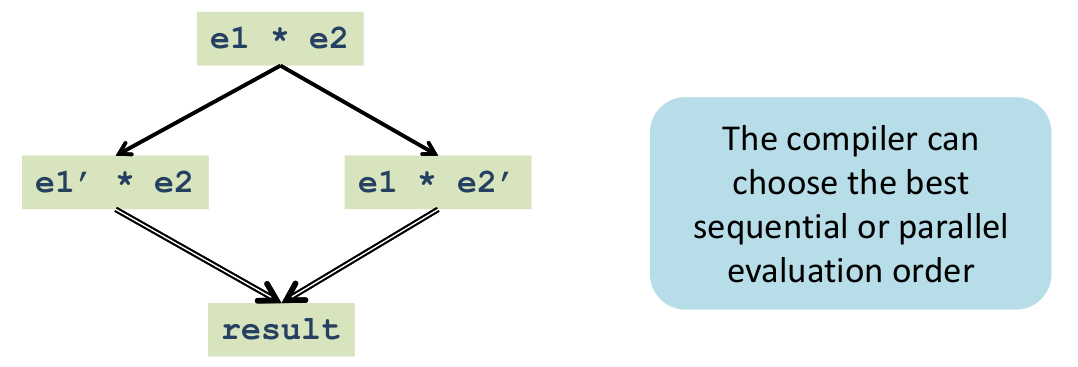
\includegraphics{images/order_eval.png}
      \caption{Evaluation order freedom}
      \label{fig:order_eval}
   \end{figure}

\labelitemize{
   \color{dkred}
   \textit{Cons}
}{
   \begin{itemize}
      \color{dkred}
      \item Input/Output
      \item Imperative update
      \item Error recovery (eg, timeout, divide by zero, etc.)
      \item Foreign-language interfaces
      \item Concurrency control
   \end{itemize}

   }
Besides, recall that the whole point of a running a program is to \textbf{interact}
with the external environment and affect it

\subsection{Towards IO}
To overcome the problem of interaction, an approach is to add imperative constructs to the language,
for instance:
\begin{lstlisting}
   res = putchar 'x' + putchar 'y'
\end{lstlisting}
Seems easy right?
Well, in fact no, because in lazy languages like Haskell,
the evaluation order is \textbf{undefined};
so, in the previous example, which char will be printed first, \lstinline|x| or \lstinline|y|?
The answer is not trivial for Haskell.
However it is not an impossible problem.
Haskell's approach is to exploit the concept of \textbf{Monads}.

Recall that the bind operator >>= forces a \textbf{sequence} between the evaluation of terms;
the IO monad exploits this and defines monadic values which are called \textbf{actions}, and prescribes how to compose
them \textit{sequentially}

\begin{figure}[htbp]
   \centering
   \begin{tikzpicture}
      % Define the styles for the rectangles
   \tikzstyle{rect} = [draw, rectangle, minimum width=4cm, minimum height=2cm, text width=3.5cm, align=center]

   % Draw the first rectangle with text A
   \node[rect] (rectA) at (0,0) {Text A\\Line 2\\Line 3};

   % Draw the second rectangle with text B
   \node[rect] (rectB) at (6,0) {Text B\\Line 2\\Line 3};

   % Draw the bidirectional double arrow between the rectangles
   \draw[-{Straight Barb[left]}] (rectA.east) -- (rectB.west);
  \draw[-{Straight Barb[right]}] (rectB.west) -- (rectA.east);
   \end{tikzpicture}
   \caption{<caption>}
   \label{<label>}
\end{figure}

\subsection*{Before Monads}
Before Monads there were \textbf{Streams}, which allowed a program to send stream of requests to OS and receive stream of responses,
or the user could supply \textbf{continuations} to I/O routines
to specify how to process results.\\
However, both of these approaches revealed to be not so useful.

\subsection{Key Ideas - Monadic I/O}

\lstinline|IO| is a type constructor, instance of \lstinline|Monad|, and a value of type \lstinline|(IO t)| is an
\textit{action} (i.e. computation) that, when \textbf{performed}, may do some
input/output before delivering a result of type \lstinline|t|
\begin{itemize}
   \item 
   \lstinline|return| returns the value without making I/O
   \item
   \lstinline|then (>>)| [and also \lstinline|\lstinline|bind (>>=)||] composes two
   actions sequentially into a larger action
   \item
   The only way to perform an action is to call it at
   some point, directly or indirectly, from
   \lstinline|Main.main|,
   which is the standard entry point for Haskell programs.
\end{itemize}

An \textbf{action} is a \textit{first-class} value,
and \textbf{evaluating} has \textit{no effect}: \textbf{performing} the
action has the \textit{effect}.
\note{The actual meaning of this statement is unclear even to the professor \smiley }

\begin{lstlisting}
   return :: a -> IO a
   return a = \w -> (a,w)
   (>>=) :: IO a -> (a -> IO b) -> IO b
   (>>=) m k = \w -> case m w of (r,w') -> k r w'
\end{lstlisting}

By writing \lstinline|case m w ...| we force the evaluation of \lstinline|m|,
resulting in the application of \lstinline|k| to \lstinline|r w'| to be performed (evaluated?) \textit{after} the evaluation of \lstinline|m|.  

\subsection{\texttt{>>=} and \texttt{>>}combinators}
Operator is called \textbf{bind} because it binds the result
of the left-hand action in the action on the right.
Performing compound action \lstinline|a >>= \x->b| :
\begin{enumerate}
   \item performs action \lstinline|a|, to yield value \lstinline|r|
   \item applies function \lstinline|\x->b| to \lstinline|r|
   \item performs the resulting action \lstinline|b{x <- r}|
   \item returns the resulting value \lstinline|v|
\end{enumerate}

\begin{figure}[htbp]
   \centering
   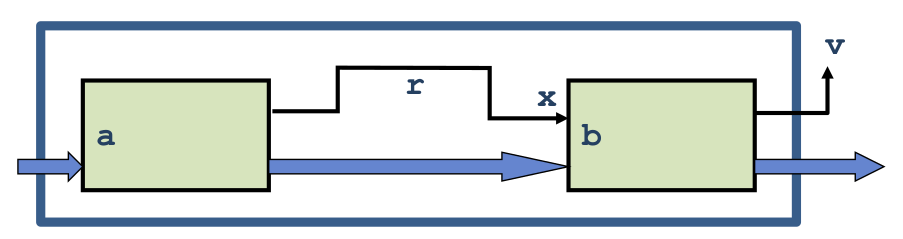
\includegraphics{images/bind_combinator.png}
   \caption{Bind Combinator}
   \label{fig:bind_combinator}
\end{figure}

The \textbf{then} combinator \lstinline|(>>)| instead does sequencing when there is no value to pass:
\begin{lstlisting}
   m >> n = m >>= (\_ -> n)
\end{lstlisting}

\subsection{Restrictions}
In pure Haskell, there is no way to transform a value of type
\lstinline|IO a| into a value of type \lstinline|a|.\\
Suppose you wanted to read a configuration file at the
beginning of your program:
\begin{lstlisting}
   configFileContents :: [String]
   configFileContents = lines (readFile "config") -- WRONG!
   useOptimisation :: Bool
   useOptimisation = "optimise" 'elem' configFileContents
\end{lstlisting}
The problem is that \lstinline|readFile| returns an \lstinline|IO String|, not a
\lstinline|String|.
\labelitemize{Possible workarounds}{
   \begin{enumerate}
      \item Write entire program in IO monad. But then we
      lose the simplicity of \textbf{pure} code.
      \item Escape from the IO Monad using a function from
      \lstinline|IO String -> String|. But this is \textbf{disallowed}!
   \end{enumerate}
}

We know the configuration file will \textit{not change}
during the program, so it doesn’t matter \textit{\textbf{when}} we
read it.\\
This situation arises sufficiently often that Haskell
implementations offer one last unsafe I/O primitive:
\lstinline|unsafePerformIO|.
\begin{lstlisting}
   unsafePerformIO :: IO a -> a
   configFileContents :: [String]
   configFileContents = lines(unsafePerformIO(readFile "config"))
\end{lstlisting}

The operator has a deliberately long name to
\textit{discourage} its use.
Besides, its use comes with a proof obligation:
a promise to the compiler that the \textit{timing} of this operation
relative to all other operations doesn’t matter.

It is called \textit{unsafe} because it breaks the soundness of the type system;
thus, claims that Haskell is type safe are valid only when \lstinline|unsafePerformIO| is \textbf{not} used.

\section{Summary}
\begin{itemize}
   \item A complete Haskell program is a single IO action called
   main. Inside IO, code is \textbf{single-threaded}.
   \item Big IO actions are built by gluing together smaller ones with
   \lstinline|bind (>>=)| and by converting pure code into actions with
   return.
   \item IO actions are first-class.
   They can be passed to functions, returned from functions, and
   stored in data structures; so, it is easy to define new "glue" combinators.
   \item The IO Monad allows Haskell to be pure while efficiently
   supporting side effects.
   \item The type system separates the \textit{pure} from the \textit{effectful} code.
\end{itemize}

\labelitemize{
   \textit{Comparison}
}{
   \begin{itemize}
      \item In languages like ML or Java, the fact that the
      language is in the IO monad is baked in to the
      language. There is no need to mark anything in the
      type system because it is everywhere.
      \item In Haskell, the programmer can choose when to live
      in the IO monad and when to live in the realm of
      pure functional programming.
      \item So it is not Haskell that lacks imperative features, but
      rather the other languages that lack the ability to
      have a statically distinguishable pure subset.
   \end{itemize}
}